\section{Scalable Vector Graphics}

%-----------------------    ---------------------------------

\begin{frame}
\frametitle{¿Qué es SVG?}

\begin{itemize}
   \item SVG es vectorial
   \item Apto para iconos e imágenes de alta calidad
   \item Puede ampliarse o reducirse sin perder calidad (esencial para la \emph{responsive web})
   \item Permite optimización gracias a la \emph{caché} de recursos gráficos
   \item Los navegadores modernos ofrecen soporte SVG nativo
\end{itemize}

\end{frame}


%-----------------------    ---------------------------------

\begin{frame}
\frametitle{El porqué de SVG visualmente}

\begin{center}
  
\includegraphics[width=10cm]{figs/svg.png}
\end{center}


\begin{flushright}
{\tiny
Source: https://commons.wikimedia.org/wiki/File:Bitmap\_VS\_SVG.svg
}
\end{flushright}

\end{frame}

%-----------------------    ---------------------------------

\begin{frame}
\frametitle{SVG}

\begin{itemize}
   \item SVG es un estándar basado en XML del W3C
   \item Permite tres tipos de objetos gráficos:
   \begin{itemize}
     \item Elementos geométricos vectoriales (p.e. caminos consistentes en rectas y curvas, y áreas limitadas por ellos)
     \item Imágenes de mapa de bits /digitales
     \item Texto
   \end{itemize}
   \item Existe un validador del W3C
   \item Hay múltiples herramientas para manipular SVGs: Inkscape, Adobe Illustrator, ...
\end{itemize}

\end{frame}

%-----------------------    ---------------------------------

\begin{frame}[fragile]
\frametitle{Ejemplo de SVG}

Un ejemplo con SVG:

\begin{footnotesize}
\begin{verbatim}
<svg xmlns="http://www.w3.org/2000/svg" version="1.1">
  <rect x="25" y="25" width="200" height="200" fill="lime"
        stroke-width="4" stroke="pink" />
  <circle cx="125" cy="125" r="75" fill="orange" />
  <polyline points="50,150 50,200 200,200 200,100" stroke="red" 
            stroke-width="4" fill="none" />
  <line x1="50" y1="50" x2="200" y2="200" stroke="blue" 
        stroke-width="4" />
</svg>
\end{verbatim}
\end{footnotesize}

\end{frame}

%-----------------------    ---------------------------------

\begin{frame}
\frametitle{Resultado visual}

\begin{center}
  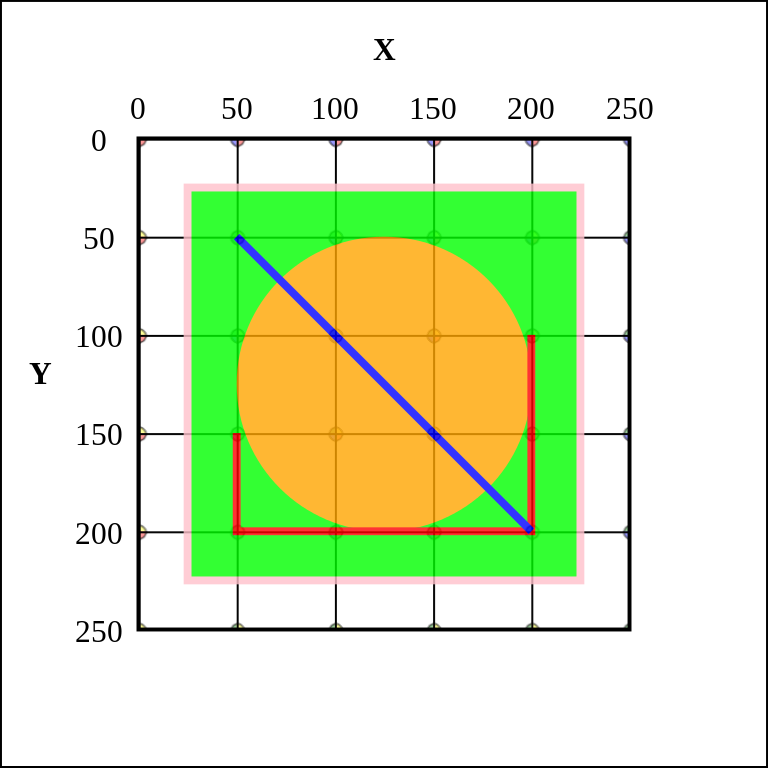
\includegraphics[width=7cm]{figs/svg-example.png}
\end{center}

\begin{flushright}
{\tiny
Source: https://commons.wikimedia.org/wiki/File:SVG\_example\_markup\_grid.svg
}
\end{flushright}

\end{frame}

